\documentclass[10pt,a4paper]{article}
\usepackage[latin1]{inputenc}
\usepackage{amsmath}
\usepackage{amsfonts}
\usepackage{hyperref}
\usepackage{amssymb}
\usepackage{graphicx}
\usepackage{kpfonts}
\usepackage{csvsimple}
\usepackage{listings}
\usepackage{subfigure}
\usepackage{graphicx}
%Styles and setups
\graphicspath{{./images/}}

\title{Activity prediction using hybrid generative/discriminative model}
\author{Lio Enrico 822861, Vasquez Alessandro 822569}
\begin{document}
\maketitle
\newpage
\section{Introduction}
In this work we want to explore the power of a particular machine learning's hybrid model, composed by a deep ANN (Artificial Neural Network) for the discriminative part and an HMM (Hidden Markov Model) for the generative part. In this hybrid model, the output of the ANN is used to refine the matrix of emission probabilities of the HMM so that the accuracy of the deep neural network is somehow ``transmitted'' to the HMM framework.
\subsection{The setting}
To train and test the hybrid model we used a dataset generated by a Wireless Sensor Network (WSN) which recorded the activation of almost a dozen sensors spread all over a user's home for a couple of weeks. The first dataset is accompanied by another dataset created from the user's annotations about which ADL (activity of daily living) was executing in which interval of time. By setting the sensors' recordings as the features and the user's ADL as the targets we can build a model that infer which sequence of ADL the user was executing by considering which sensors were activated during that period of time. 

\section{Data parsing, data alignment, data mapping}
In order to get a discretized temporal format of the dataset, we sliced the data in regularly spaced intervals of time. The chosen length of those intervals is $\Delta t=60s$.
For each $\Delta t$, we consider the first ADL being executed in that interval, whereas for the sensors we consider all sensor that were activated at least once during the considered interval. The choice of excluding other ADLs that could possibly appears in the same $\Delta t$, was made by considering that if an ADL appears as the second activity during a given interval, two scenarios are possible: in the first one the ADL is so short that will not appear in the next time interval. In this case we assume that activity to be noise and do not consider it. In the second scenario the ADL is long enough to appear as the first ADL in the next interval, and will be associated to that interval. An example of these scenarios is illustrated in figure \ref{fig:intervals}. 
\begin{figure}
	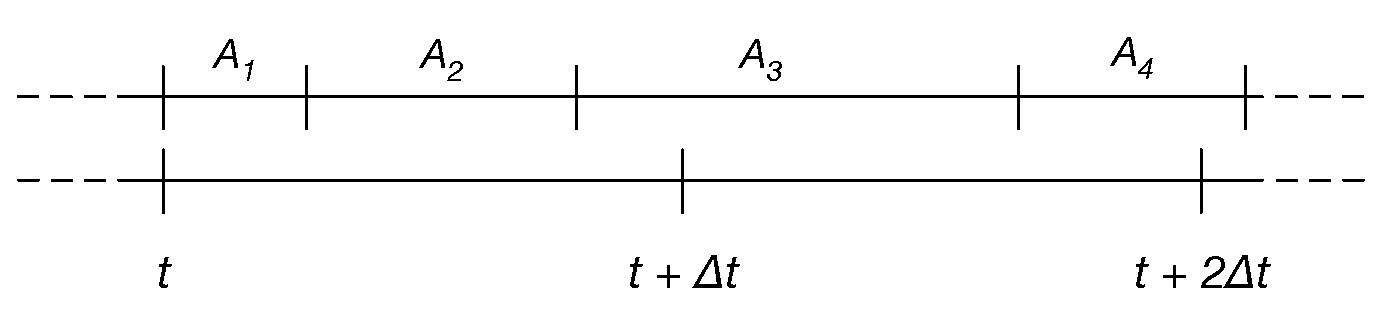
\includegraphics[ width=1.1\textwidth]{intervals.eps}
	\caption{ADLs and intervals. The activity $A_2$ being too short is considered noise and is dropped from the dataset. At the opposite, $A_3$  is long enough to be detected in next interval.}
	\label{fig:intervals}
\end{figure}
We mapped each activity and each sensor into an integer number based on the order of appearance in the dataset, such that the first activity/sensor to appear in the dataset is mapped as the $0$-th activity/sensor. This means that the mapping differs for each different dataset. In our case, two datasets were used ($A$ and $B$), thus two different mappings have been produced: \\
% mettere i csv coi mapping
\begin{center}
	\csvautotabular{csvs/labels_states_A.csv}
	\csvautotabular{csvs/labels_states_B.csv}
\end{center}


 A \textit{configuration} consists of a binary array in which the $i$-th element is set to $1$ if the $i$-th sensor activated during the given interval of time, 0 otherwise. Each observation is associated with the ADL the user was executing during that interval of time. 
 
 
\section{Hybrid model}
\subsubsection{Neural Network}
The neural network takes the configuration $y_t$ associated to the time interval $t$ as its input whereas the output, in accordance to our model, corresponds to the probability for the configuration $y$ to be observed given the state $x_{i_t}$, i.e. $p( y_t\ |\ x_{i_t}), \forall i$ at the time $t$\footnote{In the original paper the author used the Bayes rule on the output of the softmax function since they considered it the probability $p(\vec x_t\ |\ y_t)$. We made a different choice in order to not ``contaminate'' the neural network's result with the a priori probabilities of features and targets.}. The neural network's architecture is illustrated in figure \ref{fig:ann_struct}. The activation function for the hidden and the output layer is the relu function: $$relu(x)=max(0, x).$$  The \textit{softmax} function is the function $\sigma$ that transforms the logits outputted by the network in a probability distribution: $$\sigma(\vec o\ )_j = \frac{e^{o_j}}{\sum_{k=1}^{n} e^{o_k}}, \text{ for } j \in 1,..,n.$$

\begin{figure}
		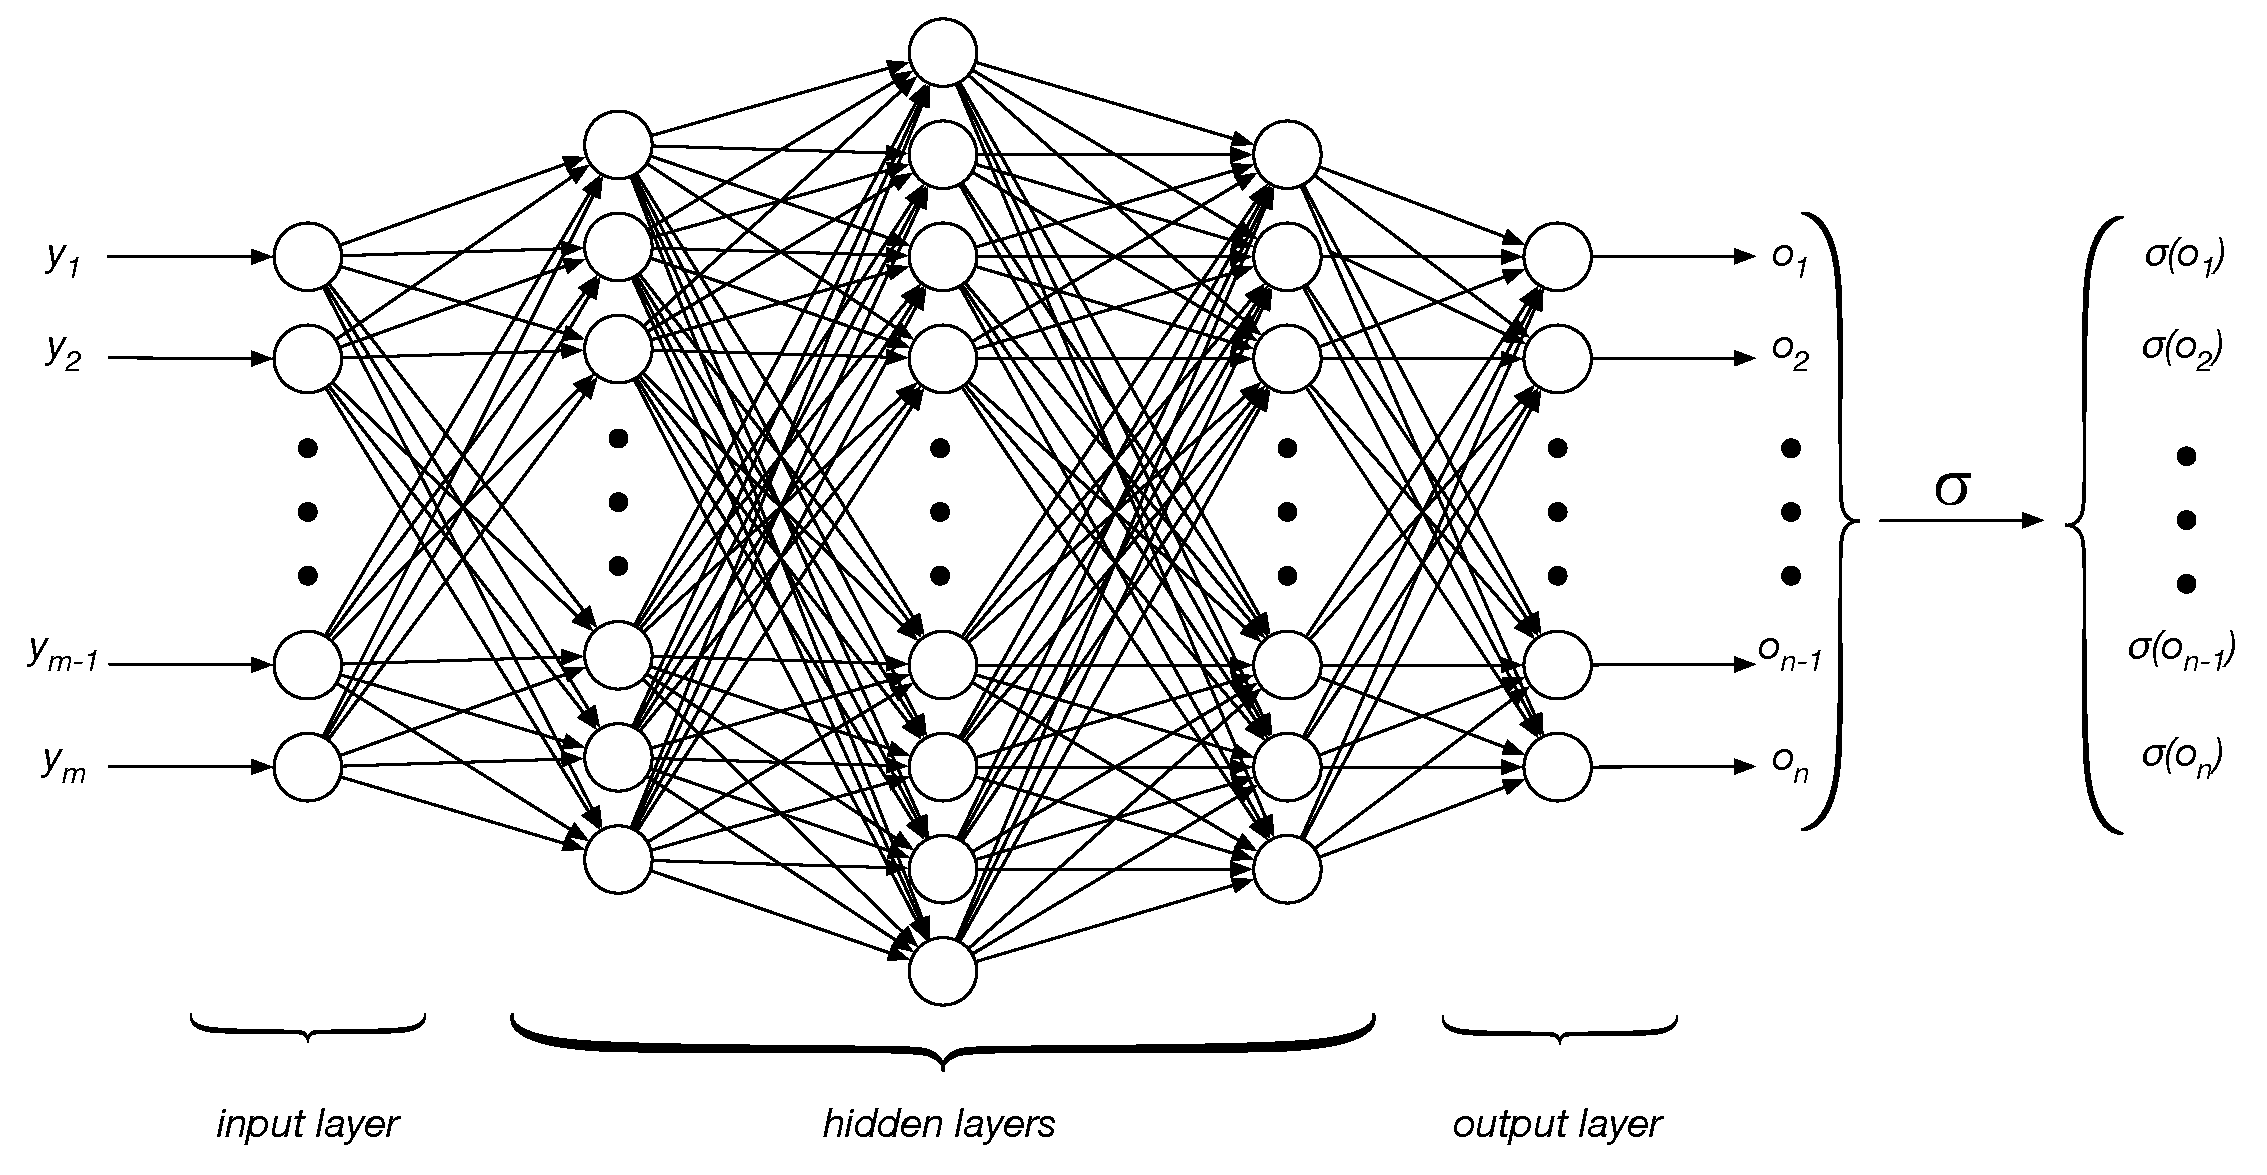
\includegraphics[ width=1.1\textwidth]{nn_struct.eps}
		\caption{Architecture of the neural network: $m$ is the number of sensors, i.e. the size of the observation's space, whereas $n$ the number of the recorded activities, i.e. the state's space.}
		\label{fig:ann_struct}
\end{figure}
\subsubsection{HMM}

\section{Implementation details}
\subsection{System's architecture}
\subsection{Third-party libraries}
We used \tt sklearn\rm, \tt numpy \rm and \tt pandas \rm for scientific computing matters. The neural network was developed with \tt keras\rm, a high-level API which uses \tt tensorflow \rm as its back-end. 
\section{Results}
Thanks to the elimination of noise in the dataset and the deep neural network contribute, we obtained predictions with a pretty nice accuracy. We used a one-day $k$-fold cross validation, in which the test set consisted of a sequence of $\thicksim 1440$ observations, the equivalent of an entire day divided by the time segments of $60$ seconds. We kept track of the average error of  both the neural network and the hybrid model. Since the neural network works on single instances at a time, we suspected that it would have outputted predictions more accurate than the hybrid model, which works on sequences of $\thicksim 1440$ elements at a time. As figure \ref{figure:err_graph} shows, we weren't so much wrong. Here, the error was computed simply by dividing the not-matched states in the sequence by the sequence's length, for each of the $\thicksim 10$ folds.

\begin{figure}
	\centering
	\subfigure[Dataset $A$.]{\label{fig:err_graph_A}\includegraphics[width=0.49\textwidth]{A/errs.eps}}
	\subfigure[Dataset $B$.]{\label{fig:err_graph_B}\includegraphics[width=0.49\textwidth]{B/errs.eps}}
	\caption{Mean error committed during testing.}
	\label{figure:err_graph}
\end{figure}
\section{Conclusions}
% how beautifuls are hybrid models

\end{document}